\documentclass[11pt,a4paper]{report}

\usepackage[utf8]{inputenc}
\usepackage[T1]{fontenc}
\usepackage[all]{xy}
\usepackage{array}
\usepackage{listings}
\usepackage[a4paper]{geometry}
\usepackage{lscape}
\usepackage{bm}
\usepackage{amsmath}
\usepackage{algorithm}
\usepackage{algorithmic}
\usepackage{tikz}
\usepackage{amsthm}
\usepackage{hyperref}
\usepackage{wrapfig}
\usepackage{xspace}
\usepackage{fancyvrb}
\usepackage{caption}
\usepackage{subcaption}
\hypersetup{
    colorlinks,
    citecolor=black,
    filecolor=black,
    linkcolor=black,
    urlcolor=black
}
\usetikzlibrary{arrows.meta}
\newtheorem{theorem}{Theorem}[chapter]
\theoremstyle{definition}
\newtheorem{example}{Example}[chapter]

\makeatletter %otherwise geometry resets everything
\Gm@restore@org
\makeatother

\setlength{\itemsep}{0cm}
\setlength{\voffset}{0cm}
\setlength{\headheight}{0cm}
\setlength{\topmargin}{0cm}
\setlength{\extrarowheight}{3pt} %for superscripts in tabular
\setlength{\arraycolsep}{4pt}

\lstset{basicstyle = \footnotesize, breaklines = true}

\graphicspath{{imgs/}}

\newfloat{lstfloat}{htbp}{lop}
\floatname{lstfloat}{Listing}

\begin{document}
\begin{titlepage}
\begin{center}
\textsc{\LARGE Internship\\Software Science}\\[1.5cm]

\includegraphics[height=100pt]{logo}

\vspace{0.4cm}
\textsc{\Large Radboud University}\\[1cm]
\hrule
\vspace{0.4cm}
\textbf{\Large Using a Hybrid Approach to Handle Complex Constraints for Product Line Configuration}\\[0.4cm]
\hrule
\vspace{2cm}
\begin{minipage}[t]{0.45\textwidth}
\begin{flushleft} \large
\textit{Author:}\\
Bob Ruiken\\
s4721306
\end{flushleft}
\end{minipage}
\begin{minipage}[t]{0.48\textwidth}
\begin{flushright} \large
\textit{First supervisor/assessor:}\\
Daniel Str{\"u}ber\\
\texttt{d.strueber@cs.ru.nl}\\[1.3cm]
\textit{Second assessor:}\\
Jan Tretmans\\
\texttt{j.tretmans@cs.ru.nl}
\end{flushright}
\end{minipage}
\vfill
{\large \today}
\end{center}
\end{titlepage}

\setcounter{tocdepth}{1}
\tableofcontents
\newpage

\setlength{\parskip}{10pt}

\chapter{Introduction}\label{ch:introduction}
Software Product Lines (SPL) are a means of creating closely related software
products by storing all of the possible features in one codebase with an
accompanying feature model that tells how the features may interact with one
another~\cite{apel2016spl, kang1990fms}. These feature models thus contain the
information needed to create \emph{valid} products. We may want to disallow
features such as \emph{Windows} and \emph{Linux} to exist at the same time, for
example. Apart from these standard relations described in feature models, we
can also have \emph{extended feature models}~\cite{benavides2005extfms}. These
feature models also contain non-functional information for features, one can
imagine that we want to add information such as performance or cost. These
non-functional parameters can later be used to guide the configuration, as to
identify a suitable feature selection - leading to a multi-objective 
optimization problem. Because
of the complexity of such models, this problem is NP-complete. The fact that
the multiple objectives are orthogonal, makes things even worse~\cite{ochoa2018npcomplete}. 

Solving this optimisation problem for feature models has been studied for more
than fifteen years and the most recent scalable solutions are all based on
meta-heuristic algorithms, specifically the genetic algorithm
IBEA~\cite{horcas2022breakit, zitzler2004ibea}. In these genetic algorithms,
activations of features are represented using bitstrings and standard mutation
and crossover operators are applied~\cite{ochoa2018npcomplete}. If one uses the
standard genetic operators, the represented selection of features is often
invalid, since it does not take the limitations of the feature model into
account~\cite{henard2015satibea, pascual2015modagame}. This requires validity
checking of solutions after applying the operators, and possibly also requires
some sort of ``fix'' operator to repair solutions. This in-situ fixing takes
time and thus hurts the performance of those algorithms. Work by Horcas et al.
mitigates this issue by creating specific genetic operators which by design do not break
the validity of configurations during changes~\cite{horcas2022breakit}. The
operators are called \emph{consistency-preserving configuration operators}
(CPCOs). These operators only have to be generated once for a feature model,
which can be efficiently done before the actual genetic algorithm is
applied~\cite{horcas2022breakit}. These CPCOs outperform the previous in-situ
fixing algorithms.

There is, however, a problem with CPCOs: the generation of
the operators is problematic for complex cross-tree constraints. Cross-tree 
constraints can be arbitrary boolean formulas to define relations between
features. CPCO generation can deal with simple ``requires'' and ``exclude'' relations,
but do not work well with general boolean formulas.

The goal of this internship is to apply a suggestion that already has been made by 
Horcas et al., where we might be able to mix the two above-discussed 
approaches. We could create CPCOs for the general case, where we have basic 
constraints and SATIBEA's~\cite{henard2015satibea} \emph{fix} operator for the 
remaining complex constraints. This might result in a situation where we have 
to do very little repairing because the CPCOs prevent most unwanted feature 
activations. This sounds like a best-of-both-words situation where we do not 
have to go through the explosive process of creating CPCOs from complex 
constraints, but we also do not have to apply the costly \emph{fix} operator 
many times. This idea requires firstly changes in the code of aCaPulCO, the 
tool created in~\cite{horcas2022breakit}. Secondly, we would like to apply the
same evaluation setup from this work again, this time also using the newly created 
variant of the algorithm.

We are going to see that while these goals seem fair and reasonable, they were
much harder to reach than initially thought. Trying to solve various
problems was the main time sink. Solving problems is a natural part of doing
research, but in this internship, the problems turned out to be unsolvable (at
least in the given timeframe of the internship.) On a more positive note, we did
manage to get a working implementation that works on limitedly sized feature models.
For these specific feature models, our implementation does not seem to have a
significant performance decrease.

The style of this document is mainly that of a research paper, describing
background information, the research process, and -- in limited form -- the
results. But we will also see that this work contains my personal experiences
with the process as a whole. Personally, I feel as if those experiences make up
a large part of the entire internship, mainly because of the problems
encountered throughout it. The outline of this work is as follows:
we start with more background, first looking into Software Product Lines and
(extended) feature models, then also looking at aCaPulCO~\cite{horcas2022breakit}
in Chapter~\ref{ch:background}.
We will then look at complex constraints and how to deal with them in
Chapter~\ref{ch:approach}. Next, we delve into the evaluation of how we can
generate test data as well as give the limited results in
Chapter~\ref{ch:evaluation} Finally, we conclude this work in 
Chapter~\ref{ch:conclusion}.
\chapter{Background}\label{ch:background}
This chapter will cover the background details of Software Product Lines
(SPLs) and extend this with Extended Feature Models. We will also 
further introduce the tool that we are working with: aCaPulCO.
\section{Software Product Lines}\label{sec:spl}
We will first give a brief introduction to \emph{Software Product Lines}.
More background details can be found in for 
example~\cite{van2001notion, apel2013software, bosch2000design}.
Software Product Lines use the same idea as age-old industrial product lines.
The idea behind them is that variants of products can be easily created when 
multiple products use the same general parts. If these parts can be created
in the same factory, we only need to combine these in different ways to create
multiple products. This idea can be read in the context of industrial
manufacturing, where we can for example create different aeroplanes that have
great overlap in their parts. We can also read this in the context of software,
this is where we talk about Software Product Lines.

Concepts used in software product lines include features, configurations,
variants and products. Since we will also use these concepts throughout this
work, let us look at them in more detail. \emph{Features} are ``\emph{a logical
unit of behaviour that is specified by a set of functional and quality
requirements}'', according to~\cite{bosch2000design}. This means that features
implement the requirements of a system, an example would be sending messages in
an e-mail system. These features can be toggled on and off, they are binary. In
source code, features can be implemented for example using \texttt{\#ifdef}
statements. \emph{Configurations} can be seen as a list of all features with
all of them either enabled or disabled. Configurations can be deemed valid with
the use of \emph{Feature Models}, which describe relations between features.
One could see how features such as \emph{Linux} and \emph{Windows} should not
occur simultaneously. \emph{Variants} or \emph{products} are configurations
applied to full systems. By applying them, certain parts in the source code can
be removed, whilst others should stay, decided by the variability mechanism
(i.e. the \texttt{\#ifdef} statements).

\begin{figure}
    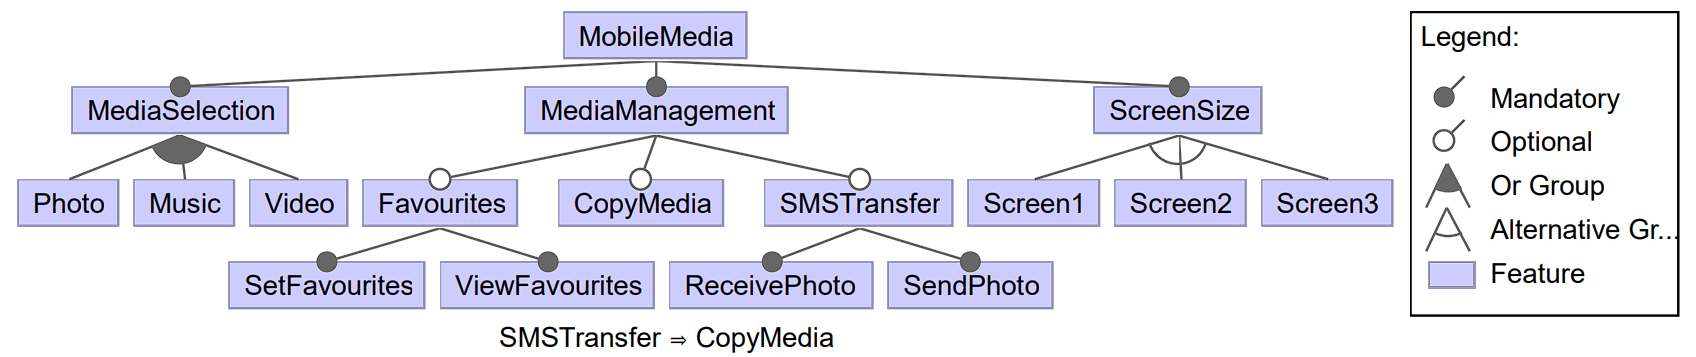
\includegraphics[width=\textwidth]{mobilemedia}
    \caption{Example Feature Model of MobileMedia}
    \label{fig:example:mobilemedia}
\end{figure}

\section{Feature Models}\label{sec:featuremodels}
Let us look at \emph{Feature Models} in more detail. As explained previously,
feature models describe relations between features. More precisely, feature
models are connected acyclic trees. The topmost feature always is a central
root feature under which other features can be placed. Growing the tree, a
hierarchy of features is created. As an example, we may have a feature
``Messaging'', which has subfeatures ``E-mail'' and ``SMS''. To be able to
create more advanced relations between features, we can place several
constraints on them. Firstly, we can define a feature to be either optional or
mandatory in relation to its parent. This would mean that (in the case of
optionality), if a parent is enabled, it is optional to enable that subfeature.
In the other case, if a parent is enabled, that child feature must also be
enabled. Of course, when we talk about something that ``must'' be the case, we
mean that the feature model is only \emph{valid} if that requirement holds.
Apart from optionality, we can also define a feature to be a \emph{group}. This
group then means that the feature designated as a group becomes the ``root'' of
that group. A group can be defined as an ``or'' group, or a ``alternative''
group. In the case of the ``or'' group, \emph{at least one} of the subfeatures of
the root of the group must be active for the feature model to hold. In
the ``alternative'' group, \emph{exactly one} of the subfeatures must be
activated.

An example feature model can be seen in Figure~\ref{fig:example:mobilemedia}.
In this feature model, we can see that the root of the model is ``MobileMedia''.
The subfeatures of this root are three mandatory features ``MediaSelection'',
``MediaManagement'' and ``ScreenSize''. The subfeatures of ``MediaSelection''
are an ``or'' group, so at least either ``Photo'', ``Music'' or ``Video'' has
to be chosen. The subfeatures of ``MediaManagement'' are optional, so they do
not have to be chosen. The subfeatures of ``ScreenSize'' are in an
``alternative'' group, which means that we need to have either ``Screen1'',
``Screen2'' or ``Screen3'', but it is limited to one of them.

We skipped over one --for us-- important detail in feature models thus far. The
example contains a boolean formula at the bottom:
\[
    \textsf{SMSTransfer} \Rightarrow \textsf{CopyMedia}
\]
These can be any boolean formula, but in this case, are limited to a simple
implication. More precisely, we would call this a ``requires'' relationship, as
the ``SMSTransfer'' feature \emph{requires} the ``CopyMedia'' feature.
These boolean formulae (there can be any number of them) must also hold, next
to the requirement of the relations defined by the tree itself. As these extra
constraints must hold for the entire tree, these boolean formulae are called
\emph{Cross-Tree Constraints}. These types of constraints will play a large
role in our research, which we will explain in more detail later.

\subsection{Extended Feature Models}\label{sec:extendedfeaturemodels}
In the introduction, we talked about feature models possibly containing 
non-functional parameters. We have seen the functional parameters in the
previous section, but have not seen non-functional parameters yet. We will
cover them here. We can include non-functional parameters in features in a
feature model, this creates a so-called
\emph{Extended Feature Model}~\cite{benavides2005extfms}. These can be
parameters such as cost and performance. We may then want to find optimal
instantiations (or products) from feature models by adding objectives to
the non-functional parameters. For example by minimising cost, or maximising
performance. Solutions are then \emph{Pareto fronts} of non-dominated
solutions~\cite{horcas2022breakit}. Finding these solutions is an NP-complete
task~\cite{ochoa2018npcomplete}, and we will go in-depth into this in the next
section.

\section{Optimising Extended Feature Models}\label{sec:tools}
In the introduction, we introduced the concept of \emph{optimising}
products in software product lines. This optimisation can only be done
in \emph{Extended Feature Models}, as they contain the relevant data
to optimise on. We know that the optimisation is NP-complete, as we want
to optimise multiple orthogonal objectives~\cite{ochoa2018npcomplete}.
A multitude of tools has been created in the past to try to solve the
optimisation problem. The most successful tools rely on genetic algorithms,
specifically the IBEA algorithm~\cite{zitzler2004ibea}. We are not going
to introduce the idea of genetic algorithms to the fullest extent here,
for more background into those, we refer you to for
example~\cite{kramer2017geneticalgos}. The basic idea is that we can
encode solutions in for example a binary bitstring. The algorithm can then
create new solutions by mutating the bitstrings (a mutation operator) and
by combining two bitstrings into one or more new solutions (a crossover 
operator). In the optimisation problem of products in software product lines,
solutions are often encoded using bitstrings as well. In those bitstrings,
a \texttt{1} represents a feature that is enabled, and a \texttt{0} 
represents a disabled feature. As long as we keep the ordering of the
features fixed, we can fully describe products using this bitstring.
In this section, we will look at how some of the state-of-the-art tools work
in more detail. We will first look at MODAGAME~\cite{pascual2015modagame}
and then look into aCaPulCO~\cite{horcas2022breakit} in even more detail, as 
we will also be working with this tool.

\subsection{MODAGAME}\label{sec:modagame}
Before we delve into how a tool such as MODAGAME~\cite{pascual2015modagame}
works exactly, we should take a look at the general way how these tools
function. The tools that we are talking about are all based on the IBEA
genetic algorithm, so we focus on those.

In genetic algorithms, we have three important phases: we first need to
select parents to create new offspring with (the \emph{selection} process),
then we create new offspring in the \emph{crossover} process, and finally
we make slight adjustments to the offspring in the \emph{mutation} process.
As mentioned before, the products are represented using bitstrings where
each bit is a feature that can be enabled (\texttt{1}), or disabled 
(\texttt{0}).

\textit{Selection} The selection process is not the most relevant
to look at for our work, the process is usually done by some standard
selection such as Binary Tournament Selection, where two individuals are
compared and the best of the two individuals is selected.

\textit{Crossover} The crossover operator should combine several parents
(usually two), to create new offspring. We can of course have multiple
different parents and children, depending on the type of crossover that we
choose. In a simple implementation such as \emph{Single-Point Crossover}, we
choose a location in the bitstring and split the (two) parents at that
location. We can then create new children by combining the bitstrings from
the first and second parents. Crossover happens at a probability decided by a 
parameter.

\textit{Mutation} A mutation operator creates more variability in the 
offspring created by the crossover operator. The mutation operator on a bitstring
can be implemented trivially. For each bit in the bitstring, we can flip each bit
at a given probability.

These three steps in a genetic algorithm work well for optimising feature models.
There is a problem, however, the simple implementation of the operators does not
keep into account the limitations we have previously put on the relations of features.
We can have for example some mandatory feature that might be disabled by a mutation
operator. Where keeping into account mandatory features is (relatively) simple,
we know that Cross-Tree constraints can contain any generic boolean formula. 
Keeping these into account during the crossover and mutation processes is very
expensive.

\textit{Fix operator} MODAGAME~\cite{pascual2015modagame} keeps these restrictions
into account in different ways. The most relevant and interesting way for us is the
\emph{fix} operator. This is another operator besides the selection, crossover and
mutation operators. It is executed after initialising solutions and after creating
new offspring. The idea of the \emph{fix} operator is that invalid representations
can be fixed during this process. One can imagine that this fixing of constraints
is expensive. In the results of MODAGAME, it is also made clear that the \emph{fix}
operator takes most of the time of the overall runtime in large feature models
(around 80\% to 90\% of the runtime.) In MODAGAME, the cross-tree constraints are
handled separately from the other constraints on the tree (such as XOR- or OR-groups).
The group constraints are repaired by enabling disabled features in an allowed manner
(i.e. by adhering to the defined groups), this is an expensive recursive operation
where enabling one feature might even lead to checking all other features. This process
will always result in a configuration that is valid to the group constraints.

The process for repairing the cross-tree constraints is different, as it is not always
guaranteed to succeed. Cross-tree constraints are often represented in CNF, where
each boolean formula is written as a conjunction of disjunctions. The \emph{fix}
operator attempts to fix invalid cross-tree constraints by attempting to fix each
disjunction separately. To fix a disjunction, we need to make one of the literals
in the disjunction positive. MODAGAME does this in a random order such that different
features are enabled every time (to increase the chance of success). Enabling the
feature is done using the same function that is used in the fixing of the group
constraints, such that enabling this feature does not break other group constraints.
It may, however, happen that other cross-tree constraints are no longer satisfied when
one of them is repaired. For this reason, the entire process of repairing cross-tree
constraints need to be restarted each time a fix is applied. This makes the repair
process for cross-tree constraints even more expensive than the previous repair process.

\subsection{aCaPulCO}\label{sec:acapulco}
Now that we have looked at how MODAGAME works, we can take a look at the tool that
we will be working with in more detail: aCaPulCO~\cite{horcas2022breakit}. The goal
of aCaPulCO was to remove the need for the \emph{fix} operator, as it slows down
the optimisation process the most. Besides slowing down the process, it also yields
incorrect solutions as the aforementioned \emph{fix} operator of MODAGAME sometimes
fails to fix the cross-tree constraints. By design, aCaPulCO does not create any
incorrect products. This section covers more details of aCaPulCO, how it works,
and also what its shortcomings are.

\emph{CPCOs} The underlying system of aCaPulCO relies on so called
\emph{Consistency-preserving configuration operators} (CPCOs). These operators
allow enabling or disabling features without breaking any constraints of the
underlying feature model. Unlike other tools, aCaPulCO can calculate these static
operators before executing the analysis part of the tool. This means that for
every feature model, the operators to enable and disable features only have to be
computed once. 

There are some principles on which the CPCO generation relies, six for the
activation of features (\emph{Activation principles}), and five for the
deactivation of features (\emph{Deactivation principles}). These are as follows
for the activation principles, where $f$ is a feature that we want to activate:
\begin{enumerate}
    \item \textsc{ActMand}: Activate all mandatory children of $f$.
    \item \textsc{ActPar}: If $g$ is the parent of $f$, and it is not activated, activate $g$.
    \item \textsc{ActReq}: If $f$ requires feature $g$, and it is not actiated, activate $g$.
    \item \textsc{ActGroup}: If $f$ is an \emph{OR} or \emph{XOR} group, activate one of the children of $f$.
    \item \textsc{ActXor}: If $f$ is one of the children of an \emph{XOR} group, deactivate all of the siblings of $f$.
    \item \textsc{ActExc}: If $f$ is excluded by, or excludes $g$, deactivate $g$.
\end{enumerate}

For the deactivation principles, we have the following, where $f$ is the feature
to be deactivated:
\begin{enumerate}
    \item \textsc{DeChild}: Deactivate all active children of $f$.
    \item \textsc{DeXor}: If $f$ is one of the children of an \emph{XOR} group, either activate one of the siblings of $f$, or deactivate its parent.
    \item \textsc{DeOr}: If $f$ is one of the children of an \emph{OR} group, either activate one of its siblings or deactivate the parent of $f$.
    \item \textsc{DeParent}: If $f$ is a mandatory feature, deactivate the parent of $f$.
    \item \textsc{DeReq}: If a feature $g$ requires $f$, deactivate $g$.
\end{enumerate}

Note that we are talking about \emph{requires} and \emph{excludes} relationships.
It should be noted that these kinds of constraints are located in the cross-tree
constraints, but these constraints are of certain shapes. The aCaPulCO tool
currently only accepts cross-tree constraints that define some requirement of a
feature (e.g. feature $f$ \emph{requires} feature $g$), or an exclusion of a
feature (e.g. feature $f$ cannot be activated when feature $g$ is active: 
$g$ \emph{excludes} $f$). In aCaPulCO, we differentiate between these constraints
(we refer to them as \emph{simple} constraints), and constraints of other shapes,
which we refer to as \emph{complex} constraints. Note that these constraints are
only relevant in the cross-tree constraints.

With the previously defined principles, we can generate sound activation and
deactivation rules for all of the features. One problem with generating the 
rules naively with just these constraints is not scalable to large feature models,
which are specifically the target of aCaPulCO. This is why an efficient algorithm
is defined for generating the CPCOs in~\cite{horcas2022breakit}. We will not cover
this algorithm in detail as it is not relevant to our work.

\begin{figure}
    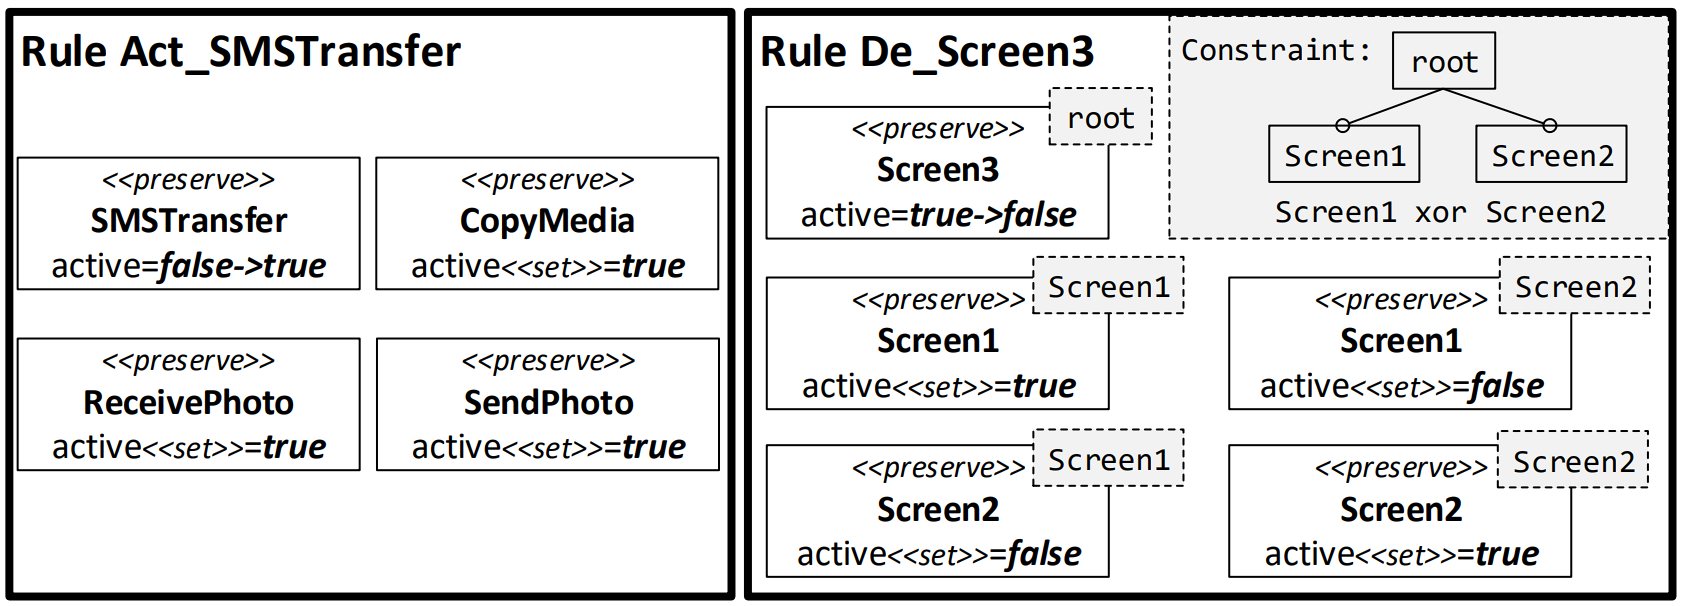
\includegraphics[width=\textwidth]{examplerules}
    \caption{Two example CPCOs for features \emph{SMSTransfer} and \emph{Screen3} of the feature model we have introduced in Figure~\ref{fig:example:mobilemedia}.}
    \label{fig:example:cpcos}
\end{figure}

Let us look at two example rules for the activation and deactivation of features
that we introduced in Figure~\ref{fig:example:mobilemedia}. We show the activation
of \emph{SMSTransfer} and the deactivation of \emph{Screen3} in 
Figure~\ref{fig:example:cpcos}. On the left, we can see the activation, where we set
\emph{SMSTransfer} to \emph{true} from \emph{false}. To do this, we also need to set
\emph{CopyMedia}, \emph{ReceivePhoto} and \emph{SendPhoto} to active. The deactivation
rule on the right is more complex. This is because the \emph{ScreenSize} feature is an
\emph{XOR} group that contains the three screen sizes. Since we want to deactivate
\emph{Screen3}, the remaining constraint is that exactly one of \emph{Screen1} and
\emph{Screen2} must be active. In the rule, we can see that we firstly set
\emph{Screen3} to \emph{false} from \emph{true}. Then we have two options, which we
label with either of the two remaining screen sizes. In one option, we enable
\emph{Screen1} and disable \emph{Screen2}, the other option is the inverse of this.

We previously mentioned how a difference is defined between two types of cross-tree constraints. We have the \emph{simple} cross tree constraints, with which
aCaPulCO can work (the CPCO generation can adhere to these rules). But we also
have \emph{complex} cross-tree constraints. The current version of aCaPulCO
cannot deal with these constraints. The reason for this is that the CPCO
generation gets too complex with the addition of these constraints. This is not
surprising, we have also seen this in MODAGAME, where the \emph{fix} operator 
will take increasingly more time when the size of the feature models is scaled
up.

To fix this, the authors of aCaPulCO already suggested going with a hybrid
approach: we keep the complex constraints out of the CPCO generation and only
take them into account in a \emph{fix} operator. This would mean that a new
processing step is added to aCaPulCO, in which only the complex constraints are
handled. Supposedly, this works better than MODAGAME, because that tool takes
care of all the types of cross-tree constraints in its \emph{fix} operator.


\chapter{Approach}\label{ch:approach}
This chapter covers more details on the approach that was taken in this research.
We will explain the details of the implementation of the \emph{fix} operator
designed to use in aCaPulCO. We will first look at the separation of the 
\emph{simple} and \emph{complex} constraints, and how they are represented in
aCaPulCO. Following that, we look at the design of the operator itself.

\section{Complex constraints}
First, recall that both the simple and complex constraints are cross-tree
constraints. Since aCaPulCO currently only accepts simple constraints in its
CPCO generation, the complex constraints are simply filtered out of the input
model. After parsing the cross-tree constraints, the arbitrary boolean formulas
are converted to CNF notation. The two accepted types of constraints 
(\emph{requires} and \emph{excludes} relationships) then look as follows:

\begin{itemize}
    \item \textit{Requires relationship}: A \emph{requires} relation is when a
          feature requires another feature for it to be enabled. We can see this
          as a logical implication, where if feature $f$ \emph{requires} feature 
          $g$, we have \( f \Rightarrow g \). Since the CNF notation only allows
          for conjunctions of disjunction, this is transformed to \( \neg f \lor g \).
    \item \textit{Excludes relationship}: An \emph{excludes} relation is when
          enabling a feature means that some other feature cannot be enabled. This
          can also be represented using a logical implication, where if feature $f$
          excludes feature $g$, we have \( f \Rightarrow \neg g \). In CNF notation
          we get \( \neg f \lor \neg g \).
\end{itemize}

In the preprocessing step for an input feature model in aCaPulCO, complex
constraints are already filtered out of the constraints. To be able to separate
the two types of constraints, we will still save the complex constraints in a
separate model. Our new \emph{fix} operator can then use this separate model to
retrieve only the complex constraints.

Now that we can distinguish the complex from the simple constraints, we can
continue onto the actual implementation of the operator itself.

\section{Fix operator}
The new \emph{fix} operator is tasked with dealing with complex constraints.
It will be called during the creation of the initial population, and after
crossover and mutation happen during the run of the genetic algorithm. This
is the same strategy as we have seen in MODAGAME~\cite{pascual2015modagame}.
The input configuration of our fix operator is a configuration which we know
is correct with the non cross-tree constraints of the feature model, as well
as the simple constraints. The strategy for fixing the constraints for the
complex constraints is very similar to the strategy used in MODAGAME. Where
MODAGAME needed to fix both the tree constraints and cross-tree constraints,
we only need to fix the cross-tree constraints.

Recall that MODAGAME fixes the cross-tree constraints by looking at all of
the input constraints and doing the following:
\begin{enumerate}
    \item If the current constraint is valid with the input configuration,
          go to the next constraint.
    \item Now we have to fix the constraint, which we can do by enabling or
          disabling exactly one feature in the constraint. This is because the
          input constraint is always a disjunction of features.
    \item If we manage to fix the constraint using one activation or
          deactivation, restart the process since we might have invalidated a previous
          constraint.
    \item If we do not manage to fix the constraint, result in failure.
\end{enumerate}

In MODAGAME, the enabling or disabling of features was quite expensive as no
information about what needs to happen to other features is stored. We 
have a simple way to enable or disable features: we have CPCOs. If we want to
enable feature \emph{A} to fix some constraint, we can simply call the CPCO for
the activation of \emph{A}.

Let us look at an example where our input configuration is as follows:
\( \left\{ \neg A, B, C, \neg D \right\} \). Now imagine we have constraints:
\(c_1: A \lor \neg B \lor D \) and \(c_2: \neg A \lor C \). 
Currently, constraint $c_1$ is invalid and is fixable
in three separate ways: we can either activate feature \emph{A} or \emph{D}, or
we can deactivate feature \emph{B}. It would be problematic to activate feature
\emph{A} however, as activating it would break constraint $c_2$. In our operator,
we randomly apply a strategy, similar to MODAGAME. We do this to not always get
stuck in the same loops (e.g. trying to activate and deactivate \emph{A} to adhere
to constraints $c_1$ and $c_2$).

\section{Limitation of approach}
This approach works, and the algorithm for fixing the constraints could even be
improved to reach success states faster. Yet there is a problem, to be able to
fix any complex cross-tree constraint, we may need to activate or deactivate any
given feature. Thus far, aCaPulCO did not require all the rules to be generated
to get results. It turns out that aCaPulCO outperforms the other
state-of-the-art tools, all the while not having generated close to all of the
CPCOs. This means that for a given feature model with for example 10.000 features,
it may only generate activation and deactivation rules for 1\% of these features.
It is of course likely that cross-tree constraints cover many features of the other
99\% of the non-generated rules. Our fix operator cannot repair those constraints,
as it can only use the rules.

One possible way of preventing this from happening might be to fix the
configurations without using the generated rules. If we do that, we manually flip
the bit in the bitstring for the appropriate feature and move on. There are two
problems with this approach:
\begin{itemize}
    \item We cannot assure that we keep true to the non cross-tree constraints, as
          we do not have functionality for that (the CPCOs made sure of this before).
    \item The crossover and mutation operators work not on the bitstrings themselves,
          but by combining rules applied to both parents. This means that the
          configurations themselves are not that important during the run of the
          algorithm. If we were to manually make changes, these changes would virtually
          be removed in the next crossover process.
\end{itemize}

Especially the second point is important for us. It would mean that during the entire
run of the algorithm, the fixes for the complex constraints are irrelevant. In that
case, we could also apply the \emph{fix} operator as the last step of the algorithm.
This is also not a real option as the \emph{fix} operator might fail, but also
because we want our genetic algorithm to keep into account these constraints. We
would not learn anything about the complex constraints if we ignore them throughout
the process.

\chapter{Evaluation}\label{ch:evaluation}
This chapter covers the evaluation of the implemented operator. The quantifiable
results are minimal, because of the problems of the approach mentioned previously.
This chapter first starts with some notes on the generation of test data, and the
difficulties that come with it. We then briefly give some results on the time
taken by our implemented \emph{fix} operator.

\section{(Generation of) Test Data}\label{sec:testdata}
After the discovery of the aforementioned problems with the implementation of the
\emph{fix} operator in the current version of aCaPulCO, it should be clear that
we cannot test the large feature models that were used to evaluate the tool without
the \emph{fix} operator. These large feature models such as \emph{Linux} and
\emph{Automotive} (which are common feature models used to benchmark tools) are
simply too large to be able to generate all the CPCOs. For the small feature models,
we already have several other tools that can handle them. This means that we
need to get ahold of more input data.

To be able to control certain parameters in feature model generation, we could use
a tool such as BeTTy~\cite{segura2012betty} (BEnchmarking and TesTing on the analYsis
of feature models). It is a highly configurable tool that can be used to generate
(extended) feature models, it is easy to use parallel to aCaPulCO, as it is also
written in Java.

Because we want to benchmark specifically our \emph{fix} operator, we want to
generate feature models with many cross-tree constraints. Specifically, we want to
generate \emph{complex} cross-tree constraints. It should be clear that a feature
model with many cross-tree constraints would also need many features. If we have
a limited number of features, it is difficult to generate cross-tree constraints
that do not invalidate other constraints. We also do not want cross-tree constraints
to create dead features (features that can never be active), or false optional 
features (features that should be optional but are made mandatory because of
added constraints). For a tool such as BeTTy to create feature models that adhere
to these requirements, as well as a large number of cross-tree constraints, it needs
to generate large feature models with thousands of features. This brings us back to
our initial problem, where we did not want such large models, as it is not feasible
to generate all the CPCOs for them.

Apart from the difficulty of generating valid cross-tree constraints, it should
also be noted that a tool such as BeTTy can only generate simple constraints: it
is limited to creating \emph{requires} and \emph{excludes} relationships. For us,
this is not useful as aCaPulCO already can deal with these.
What we can do to prevent this, is to generate simple constraints and mark them
as complex constraints. With this approach, we do not solve the problem of the
generation that we mentioned previously.

To create the models that are used for our results, we let BeTTy generate models
with an increasing number of constraints. We limited the number of features to
a hundred, to prevent not being able to finish CPCO generation. The number of
complex constraints was set between 10\% and 45\% (in terms of the number of features).
BeTTy generates feature models that are not directly supported by aCaPulCO, because
of formatting differences, to solve this, they can first be opened in FeatureIDE~\footnote{\url{https://www.featureide.de/}}.
We already mentioned that BeTTy generates constraints that will result in dead
or false-optional features, these problems were solved by hand, also in FeatureIDE.

\section{Results}\label{sec:results}
In the previous sections, we realised that our \emph{fix} operator is not a good
fit for the current version of aCaPulCO, as it requires all the CPCO rules to be
generated, while the other operators in aCaPulCO do not have this requirement.
The smaller feature models that were benchmarked in the previous work on aCaPulCO
do not have to be benchmarked again with the \emph{fix} operator enabled, as these
small feature models do not contain any complex cross-tree constraints at all. That
would mean that our new operator does not get any work at all.

As we mentioned before, we did generate a number of smaller feature models containing
complex constraints. The results from these feature models can be found in Table~\ref{tab:results}.
In the table, we can see for each model: the number of features, the number of constraints
(\emph{S} for simple- and \emph{C} for complex constraints). Then we see the runtime
comparison between not having the fix operator and the runtime including the constraints
and fix operator. In the last column we can see the number of times a fix had to be
applied by the operator. The results were generated by running each model ten times, and taking the median of
the runtimes and application count.

The number of features is increased from what we described earlier (118 instead of 100),
this is because of the format change we had to apply, this increased the number of features
by creating separate features for group constraints. The simple constraints are all
non cross-tree-constraints: they make up the group constaints and mandatory feature
constarints. It should also be noted that the number of complex constraints is significantly
lower than expected. In the ideal case, this number should match the number in the model
name. The decrease is explained by the fact that we had to remove constraints manually
to fix inconsistencies created by them (they created false-optional or dead features).

The difference in runtime the fix operator brings is about a 10\% increase. The number
of times a fix had to be applied does not seem to bring a significant change to the
increase in runtime. The number of times the fix operator had to be applied does not
seem to corrolate strongly with the number of complex constraints in a model. The
seemingly random differences in both the runtime and fix count can be explained by both
the randomness of the algorithm and the fact that we are working with relatively small
models.

\begin{landscape}
\begin{table}[H]
    \centering
    \caption{Table showing the results of the feature models generated by BeTTy}
    \label{tab:results}
    \begin{tabular}{l|lll|ll|l}
        Model & \# Features & \# Constraints (S) & \# Constraints (C) & Runtime (no fix) & Runtime (with fix) & Fix count \\ \hline \hline
        Model10 & 118 & 201 & 5 & 197ms & 216ms & 142 \\
        model15 & 118 & 200 & 10 & 183ms & 196ms & 110 \\
        model20 & 118 & 200 & 13 & 186ms & 203ms & 127 \\
        model25 & 118 & 200 & 16 & 185ms & 202ms & 169 \\ 
        model35 & 118 & 200 & 23 & 191ms & 217ms & 284 \\
        model40 & 118 & 200 & 25 & 187ms & 215ms & 181 \\ 
        model45 & 118 & 200 & 28 & 199ms & 225ms & 230 \\
    \end{tabular}
\end{table}
\end{landscape}

\chapter{Conclusion}\label{ch:conclusion}
The goal of this research was to create a hybrid approach to deal with
complex constraints parallel to the CPCOs in aCaPulCO. In the process of
creating this operator and doing the research, it became clear that this
approach does not work for aCaPulCO. This is because aCaPulCO, in its
current state, can work with an incomplete rule generation. The \emph{fix}
operator that we implemented cannot work with this incompleteness.

The conclusion that we \emph{can} draw from this research, is that feature
models are complex, and deal with any type of cross-tree constraint
makes analysis prohibitively expensive. We also see this cost in the
generation of test data, where it is difficult to generate suitable cross
tree constraints on the fly. 

The scope of this internship is mainly limited by time, and a lot of time
has been put into trying to make the operator (in its current form) work.
When the limitation was identified, there was not enough time to delve into
the generation of the CPCOs, to try to make it more efficient (the current
limitation of the generation is explosive memory usage). This means that
after the discovery of the limitation, the focus was put on trying to find
the actual limits of the \emph{fix} operator. The idea here was to generate
suitable feature models, using BeTTy. This also turned out to be a timesink 
that did not yield positive results, because of the problems mentioned in
the previous chapter.

To make aCaPulCO work with complex cross-tree constraints, there are multiple
ways to go in future work. It is possible to look into the current form of
the CPCO generation and try to solve the memory issues in it. It could also
be interesting to further look into other ways of repairing the cross-tree
constraints, without the need for all of the CPCO rules to be generated. 


\bibliographystyle{plain}
\bibliography{bibliography}

\end{document}
\endinput
